
%  Copyright 2020-2026 Robert Bosch GmbH
%
%  Licensed under the Apache License, Version 2.0 (the "License");
%  you may not use this file except in compliance with the License.
%  You may obtain a copy of the License at
%
%      http://www.apache.org/licenses/LICENSE-2.0
%
%  Unless required by applicable law or agreed to in writing, software
%  distributed under the License is distributed on an "AS IS" BASIS,
%  WITHOUT WARRANTIES OR CONDITIONS OF ANY KIND, either express or implied.
%  See the License for the specific language governing permissions and
%  limitations under the License.

\section{Working Modes}
Roo Code uses specialized personas to optimize token usage and task accuracy.

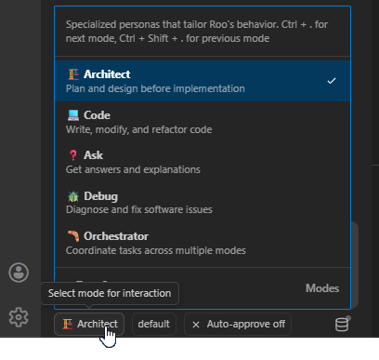
\includegraphics{./include/graphics/roocode/RooCodeModes.png}

\begin{itemize}
   \item \textbf{Architect:}
      \begin{itemize}
         \item \textbf{Goal:} Planning and high-level design.
         \item \textbf{Behavior:} Proposes solutions and analyzes code without
            making changes.
      \end{itemize}
   \item \textbf{Code:}
      \begin{itemize}
         \item \textbf{Goal:} Full implementation.
         \item \textbf{Behavior:} Has full write-access to create features,
            refactor code, and update the workspace.
      \end{itemize}
   \item \textbf{Debug:}
      \begin{itemize}
         \item \textbf{Goal:} Bug hunting and fixing.
         \item \textbf{Behavior:} Specifically designed to analyze logs,
            terminal errors, and fix broken test scripts.
      \end{itemize}
   \item \textbf{Orchestrator:}
      \begin{itemize}
         \item \textbf{Goal:} Complex task management.
         \item \textbf{Behavior:} Breaks down large objectives into smaller
            sub-tasks for execution.
      \end{itemize}
   \item \textbf{Ask:}
      \begin{itemize}
         \item \textbf{Goal:} Knowledge retrieval.
         \item \textbf{Behavior:} Acts as a read-only consultant to explain
            logic or query documentation.
      \end{itemize}
\end{itemize}

\section{Best Practices for Automation Engineers}
\begin{itemize}
   \item \textbf{Context Management:}
      Keep only relevant files open to reduce token costs.
   \item \textbf{Terminal Verification:}
      Always let Roo Code run your Robot Framework commands
      (e.g., \plog{robot path/to/test.robot}) to verify its own fixes.
   \item \textbf{Approval Workflow:}
      Carefully review the \textbf{Diff} view before clicking \textbf{"Approve"}
      to ensure the accuracy of file changes.
\end{itemize}

\section{References}
For more information and detailed documentation,
refer to the following resources:
\begin{itemize}
   \item \textbf{Roo Code Homepage:}
      \href{https://docs.roocode.com/}{docs.roocode.com}
   \item \textbf{Roo Code Tutorial Videos:}
      \href{https://docs.roocode.com/tutorial-videos}
      {https://docs.roocode.com/tutorial-videos}
   \item \textbf{Roo Code Example - First Task:}
      \href{https://docs.roocode.com/getting-started/your-first-task}
      {https://docs.roocode.com/getting-started/your-first-task}
   \item \textbf{MCP Directory:}
      \href{https://modelcontextprotocol.io/}{Model Context Protocol}
\end{itemize}
